% 1991 年上海卷第 27 题：△ABC 的三边及 ∠ACB（依固定扫描页重绘，只画拓扑与标号，不按比例）
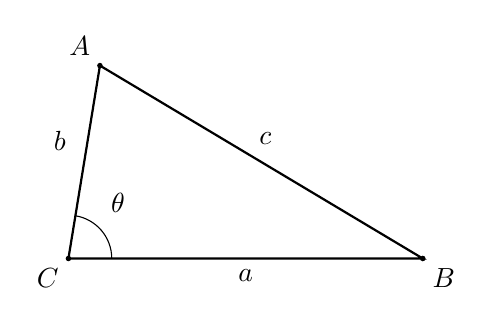
\begin{tikzpicture}[>=stealth,scale=1.0]
  \coordinate (A) at (-1.55,2.15);
  \coordinate (C) at (-1.95,-0.30);
  \coordinate (B) at (2.55,-0.30);
  \draw[thick] (A)--(C)--(B)--cycle;
  % 角 θ（顶点 C，介于 CA 与 CB 之间）
  \draw (C) ++(0:0.55) arc (0:81:0.55);
  \node at (-1.32,0.40) {$\theta$};
  \node[below] at (0.30,-0.32) {$a$};
  \node[above left] at (-1.86,0.95) {$b$};
  \node[above] at (0.55,1.02) {$c$};
  \fill (A) circle (1pt) node[above left] {$A$};
  \fill (C) circle (1pt) node[below left] {$C$};
  \fill (B) circle (1pt) node[below right] {$B$};
\end{tikzpicture}
